%!TEX root = Literature_Review_David_Burns.tex
\chapter{Modelling}
\label{ch:model}

Given the nebulous problems in atmospheric science, the best way of obtaining a theoretical description of the systems is through modelling. Generally, a number of models are chained together to simulate different parts of the climate system. Each of these models is built upon a number of theories that are used depending on the state of the system at the time \citep[Chapter 21]{jacobson2005fundamentals}. This makes atmospheric modelling difficult and broad. Fortunately many models have been developed around the world to fill various niches \citep{draxler:1997tga, mann:2010wb, cope:2009tz, mcgregor2008updated}.

The first choice to make when deciding which model to use is between a Global Climate Model (\gls{gcm}) and a Regional Climate Model (\gls{rcm}). The difference is in the granularity achieved in the discretisation used to solve the governing equations, and the requirements of boundary conditions \citep{thatcher:2015wy}. A \gls{rcm} is run on a smaller scale for a specific region with a high density of grid points. As only a small portion of the Earth's surface is simulated, the values of parameters at the boundary of that region must be known in advance \citep{hurley2002air}. Usually these boundary conditions are obtained from a previous run of a \gls{gcm}. Although a \gls{gcm} is less restrictive than a \gls{rcm}, its lack of high resolution may miss small but critical details. Conversely, the regional restriction of a \gls{rcm} can miss distant events that may influence the climate in the simulated region \citep[Chapter 25]{seinfeld2012atmospheric}.

% 'one short paragraph on this'
% What are the base equations most models use?
% Reduced versions of the navier stokes eqns...
% What ways can we numerically solve these equations?
% finite difference
% finite element
% operator splitting
% finite volume?
% 'include a sentence from this in the above paragraph to illustrate approximations'
% Obviously the full blown navier stokes equations are far too complicated to solve. So what approximations are generally used by climate modellers to still encapsulate some of the more complicated flow dynamics?
% An example is eddy diffusivity. Eddy currents occur on both small and large scales and are the result of turbulent flow around obstacles such as land masses 'cite'. A constant called the eddy diffusivity attempts to cover mixing due to eddy currents. I think this is a good example of the limitations in atmospheric models and attempts to use simple equations to approximate more complex phenomena.
% Actually it seems like most models neglect normal diffusion in favour of turbulent diffusion as the rate of turbulent diffusion dominates regular diffusion \citep[Chapter 17]{seinfeld2012atmospheric}.


% Whats the difference between eulerian and lagrangian modelling?
% What is semi-lagrangian modelling? benefits?


% what is sensitivity to initial conditons and what effect does this have on models?
% How can we tell when models are accurate?
% What methods should we use to decide if the model is good? (this is before data is taken so i mean things like sensitivity analysis), cite examples of things like sensitivity analysis, switching various things on and off to understand what is happening.


%--------------------------------------------------------------------------------------------------------------------------%
%--------------------------------------------------------------------------------------------------------------------------%

	\section{Back Trajectory Modelling}
	\label{sec:backtraj}

	When working in atmospheric science, it is often necessary to produce an idea of where a particular parcel of air has travelled from. With the advent of large scale meteorological measurements, the data required to model this process is now being produced. Trajectory modelling is able to take a particular location and predict, forward or backward in time, the path a parcel of air travels to or from that location. It can be used to predict whether air at a particular location has passed over a region or event of interest or, for example, whether there has been contamination from anthropogenic sources \citep{draxler:1998vr}.

	\gls{hysplit} is the Hybrid Single Particle Lagrangian Integrated Trajectory model developed by the National Oceanic and Atmospheric Administration and Australia's Bureau of Meteorology. It takes as input a variety of different meteorological data sources to produce the field the parcel travels through. \gls{hysplit}'s efficacy in performing back trajectory modelling is well established \citep{draxler:1998vr}. It has been used to model many different scenarios from forecasting fire smoke movement \citep{rolph:2010in} to nuclear cloud dispersion \citep{rolph:2014kk}.

	A Lagrangian model may be implemented in two different ways. A puff model regularly releases and follows a parcel of air containing the required fraction of trace components. The puff moves and expands depending on advection and diffusion respectively. A particle model releases many single particles which are moved through advection, but which are also randomly moved based on the diffusion present \citep{draxler:1997tga}. \gls{hysplit} implements a hybridisation of these models by using the particle style for vertical motion, and the puff style for horizontal motion \citep{hurley:1994df}.

	%The user provides a location and time for the start of the trajectory, and the amount of time backwards or forwards for it to run. \gls{hysplit} produces a line of lattitude and longitude points where each point is an amount of time away from the starting time. Thus the line through the points indicates the trajectory, backwards or forwards through time of the air at the starting location. 'is this too much like the first paragraph?'

	\gls{hysplit}, like all atmospheric models, is sensitive to initial conditions \citep{challa2008sensitivity} and its accuracy is dependent on the error margins of the meteorological data it makes use of \citep{draxler:1998vr}. The results of any trajectory run are therefore less accurate the further away from the initial conditions the trajectory gets. There is also a dependence on the spatial and temporal granularity of the meteorological data. As such, \gls{hysplit} offers the ability to slightly permute the initial conditions of the model to produce a multitude of possible trajectories for a single location and time \citep{draxler:1997tga}. It is also possible to produce multiple trajectories over time or over space and a robust scripting platform exists to allow this \citep{draxler:1997tga}.

	% I think we should keep this for the section where we actually do work...

	% \subsection{\gls{hysplit} Visualisations}
	% \label{subsec:hysvis}

	% 	A technique for producing meaningful visualisations of this modelling system, given it's shortcomings, is to produce a probability density function of multiple potential trajectories. The GUI side of \gls{hysplit} offers a method for doing this using the bulk production of trajectories from permuted initial conditions \citep{draxler:1997tga}.  A spatial domain is subdivided into boxes, then whatever points of the various trajectories that lie in that box are counted. Each box is then normalised by the total number of trajectory points in the domain. It is then possible to plot these boxes onto a map of the region, colouring them based on their values. This technique provides a visual idea of the probability that a given parcel of air will have passed over that box. Similarly, by producing multiple trajectories over time, it is possible to create a visualisation of the probability a parcel of air has passed through a box within a time period. 'should i put an example here?'
	% 	'should i talk about plotting the exact trajs and then animating it over time?'
	% 	If the number of points in box $i$ is $N_i$ then the probability of the parcel of air being in that box $p_i$ is given by,
	% 	\begin{align}
	% 		p_i = \frac{N_i}{\sum_{i=1}^m N_i},
	% 	\end{align}
	% 	where $m$ is the total number of boxes \cite[Chapter 3]{Lefebvre:2006vi}.

	% 	Another visualisation tool is to create a time series of the trajectories, overlaid on a map, in a movie. This shows how the trajectory evolves with the changing meteorological conditions. This could be coupled with \gls{pdf}s computed using small variations of the initial conditions to produce a better idea of probable trajectories' evolution through time.




%--------------------------------------------------------------------------------------------------------------------------%
%--------------------------------------------------------------------------------------------------------------------------%

	% \section{Unified Model}
	% \label{sec:unimod}
	% 'contemplate dumping this paragraph'

	% The Unified Model (\gls{um}) is a suite of models produced by the United Kingdom Met Office. One of the submodels for dealing with chemistry and aerosols is the United Kingdom Chemistry \& Aerosols model \gls{ukca}. One of the aerosol sub models for \gls{ukca} is \gls{glomapm}. This is a version of a combined meteorological, chemical, and aerosol model with feedback throughout the submodels 'site some unified model description paper'.

%--------------------------------------------------------------------------------------------------------------------------%
%--------------------------------------------------------------------------------------------------------------------------%

	\section{CCAM, CTM, GLOMAP}
	\label{sec:ccg}

	The three models to be used in this project are \gls{ccam}, \gls{ctm} and \gls{glomapm}. \gls{ccam} provides the meteorological data needed for \gls{ctm} and \gls{ctm} provides the chemical concentration data required for \gls{glomapm}. However, currently the system is limited to running \gls{ccam} offline from the other models (see \cref{fig:modelstruct}) \citep{mcgregor2008updated}. Thus there is no feedback into the meteorology from changes in aerosol levels, such as cloud production caused by changes in \gls{ccn} concentrations.

	\begin{figure}[!htb]
	    \centering
	    \vspace*{5mm}
	    \includegraphics[width=0.8\textwidth]{Fig/ModelStructure.tikz}
	    \vspace*{5mm}
	    \caption{The group of models prepared by \gls{csiro} for modelling from meteorology to aerosols. Arrows indicate the direction data passes.}
	    \label{fig:modelstruct}
	\end{figure}

	This combination of models has been used previously in the Sydney Particle Study \citep{cope:2014tw}. The Sydney Particle Study was a large scale study performed by seven different organisations and lead by CSIRO. It encompassed both measurement and modelling of fine particles in the Sydney area, with a view to understand their exposure to Sydney's population. Both \gls{ccam} and \gls{tapm} (an alternative meteorological model produced by \gls{csiro}) were used as the \gls{rcm}s for the study. Their outputs were compared with each other, and with the collected data. \gls{ctm}, and consequently \gls{glomapm}, were used for the particle dynamics and chemical transport modelling within the two \gls{rcm}s. Both \gls{rcm}s performed well, with predictions of sea salt, organic matter and secondary inorganic aerosols within \SI{15}{\percent} of observations (see \cref{fig:sydpartdata}) \citep{cope:2014tw}.

	\begin{figure}[!htb]
	    \centering
	    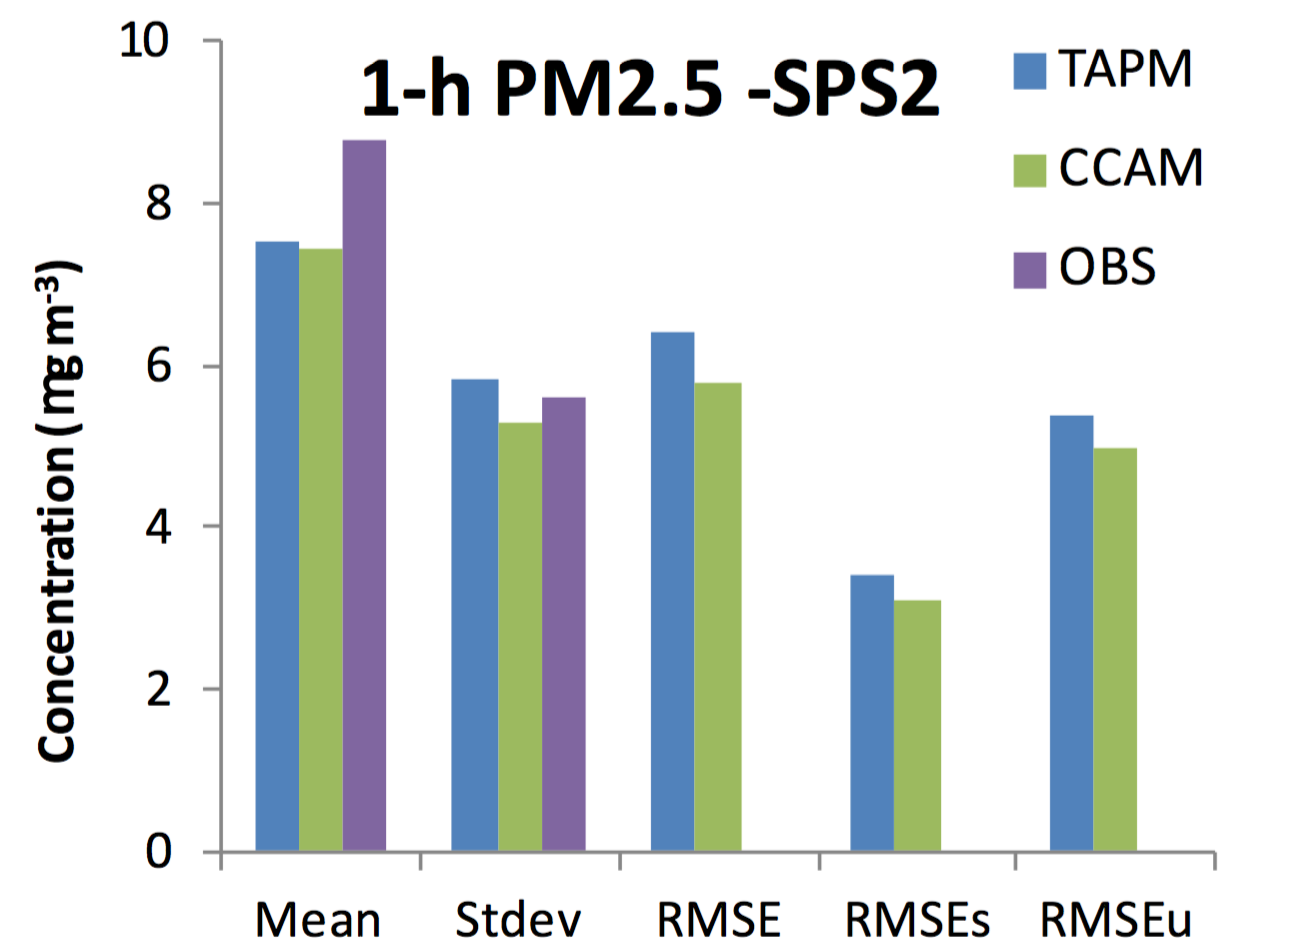
\includegraphics[width=0.6\textwidth,natwidth=1308,natheight=952]{Fig/sydneyparticledata.png}
	    \caption{The hourly averaged concentrations of PM2.5 particles for the second Sydney Particle Study. Both \gls{ccam} and \gls{tapm} used as the base meteorological model produce similar average concentrations, close to observation \citep{cope:2014tw}.}
	    \label{fig:sydpartdata}
	\end{figure}




%--------------------------------------------------------------------------------------------------------------------------%

		\subsection{CCAM}
		\label{subsec:ccam}

		\gls{ccam} is \gls{csiro}'s Conformal-Cubic Atmospheric Model. Most \gls{rcm}s are performed on a grid that simulates only the area of interest, requiring spatial boundary conditions to be fed into the model at each time step \citep{hurley2002air}. Because of \gls{ccam}'s approach of conformal cubic mapping, the majority of grid points can be focussed onto the region of interest while still simulating the rest of the globe with a gradient of accuracy (see \cref{fig:ccammap}). This removes the necessity for boundary conditions as the full globe is being simulated. This allows distant events to influence the region of interest. However, there are fewer grid points in distant regions, sacrificing accuracy for computation time \citep{mcgregor:2005wz}.

		\begin{figure}[!htb]
	    	\centering	    

  			\begin{subfigure}[b]{0.8\textwidth}
  				\centering
	    		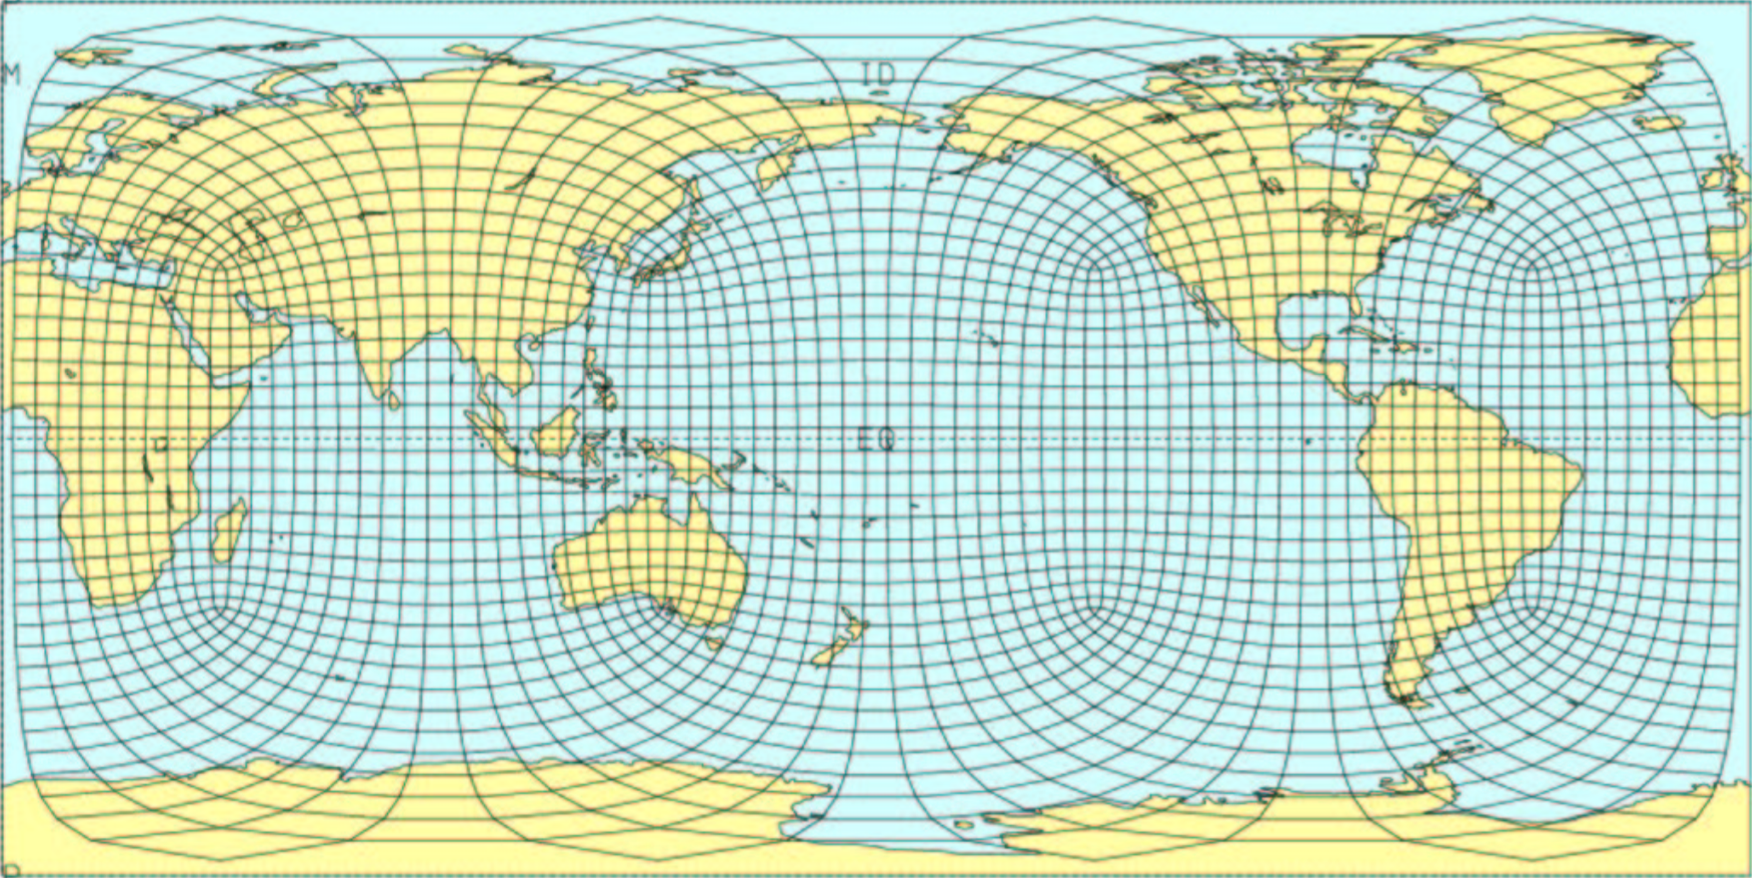
\includegraphics[width=\textwidth,natwidth=1752,natheight=878]{Fig/ccamnormal.png}
   				\caption{}
   				\label{fig:ccammapnorm} 
			\end{subfigure}

			\begin{subfigure}[b]{0.8\textwidth}
			\centering
	    		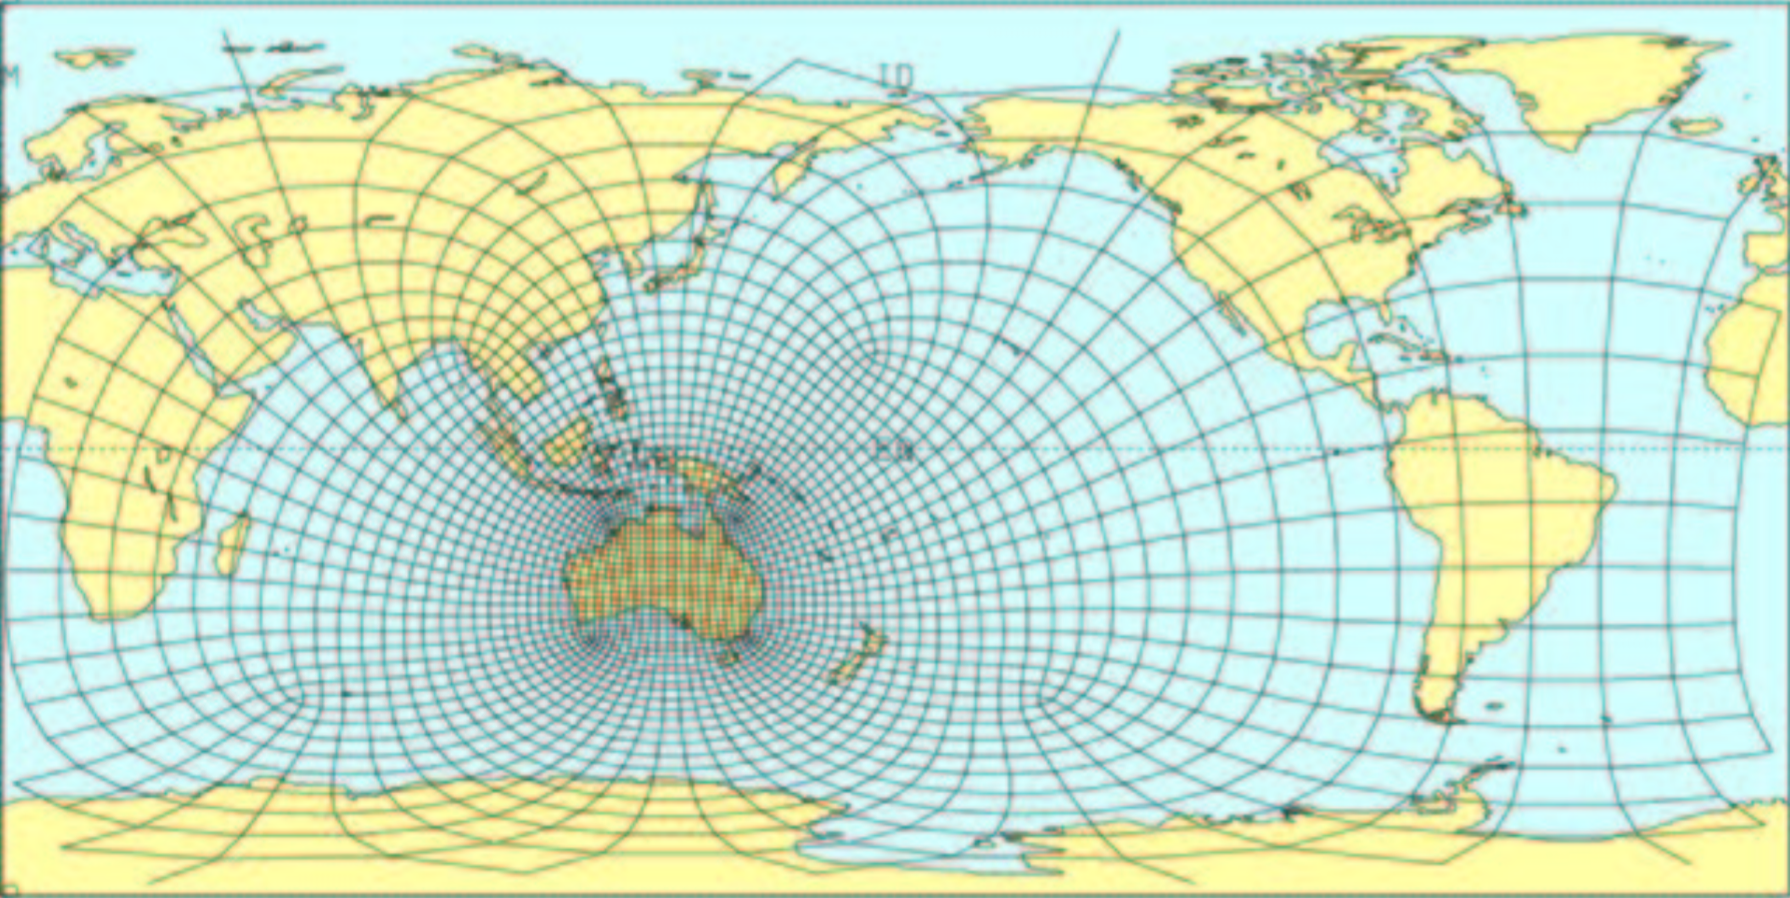
\includegraphics[width=\textwidth,natwidth=1790,natheight=898]{Fig/ccamfocussed.png}
				\caption{}
				\label{fig:ccammapfocus}
			\end{subfigure}

			\caption{Two examples of the conformal cubic mapping, used by \gls{ccam}, showing both a focussed and unfocussed transformation of the grid \citep{mcgregor:2005wz}.}
	    	\label{fig:ccammap}
		\end{figure}

		%The cubic grid structure creates a number of numerical problems. The most obvious is the existence of singularities at the corners. 'I think ccams semi-lagrangian approach helps here, and some paramters are treated differently... this is all in the ccam description papers but i dont understand it yet'

		As inputs \gls{ccam} can accept data sets from a \gls{gcm} and nudge the model towards these values \citep{mcgregor:2005wz}. Although work is being done to incorporate a coupled ocean model with matching grid structures, without this the oceanic parameters, such as sea surface temperature, must be input as both spatially and temporally varying maps \citep{mcgregor2008updated}. Despite the non-uniformity of the cubic grid structure, \gls{ccam} produces latitude and longitude based output through interpolation of the cubic grid data \citep{thatcher:2015wy}.

		The current implementation of \gls{ccam} uses a semi-Lagrangian solver that is semi-implicit and non-hydrostatic, programmed in FORTAN. The solver is designed for expansion to a large number of cores, while dealing with the singularity-like points caused by the cubic mapping \citep{thatcher:2015wy}. It is also possible to run the model multiple times, focussing the grid in at each step while nudging is performed using the previous runs' data \citep{mcgregor2008updated}.


%--------------------------------------------------------------------------------------------------------------------------%

		\subsection{CTM}
		\label{subsec:ctm}

		\gls{ctm} is the Chemical Transport Model produced at \gls{csiro}. It deals with various transport processes relating to chemicals found in the atmosphere, as well as deposition onto particles, changes in chemical structure, and emission sources \citep{cope:2009tz}. It uses a regular grid structure which requires boundary conditions (see \cref{fig:sydpartgrid}) that are usually taken from a \gls{gcm} \citep{cope:2014tw}. The transport of each chemical species is modelled using an advection diffusion equation around the chemical's concentration, with source terms relating to different chemical processes. Each of these are themselves modelled and solved before being fed back into the advection diffusion solver \citep{cope:2009tz}. 

		\begin{figure}[!htb]
	    	\centering
	    	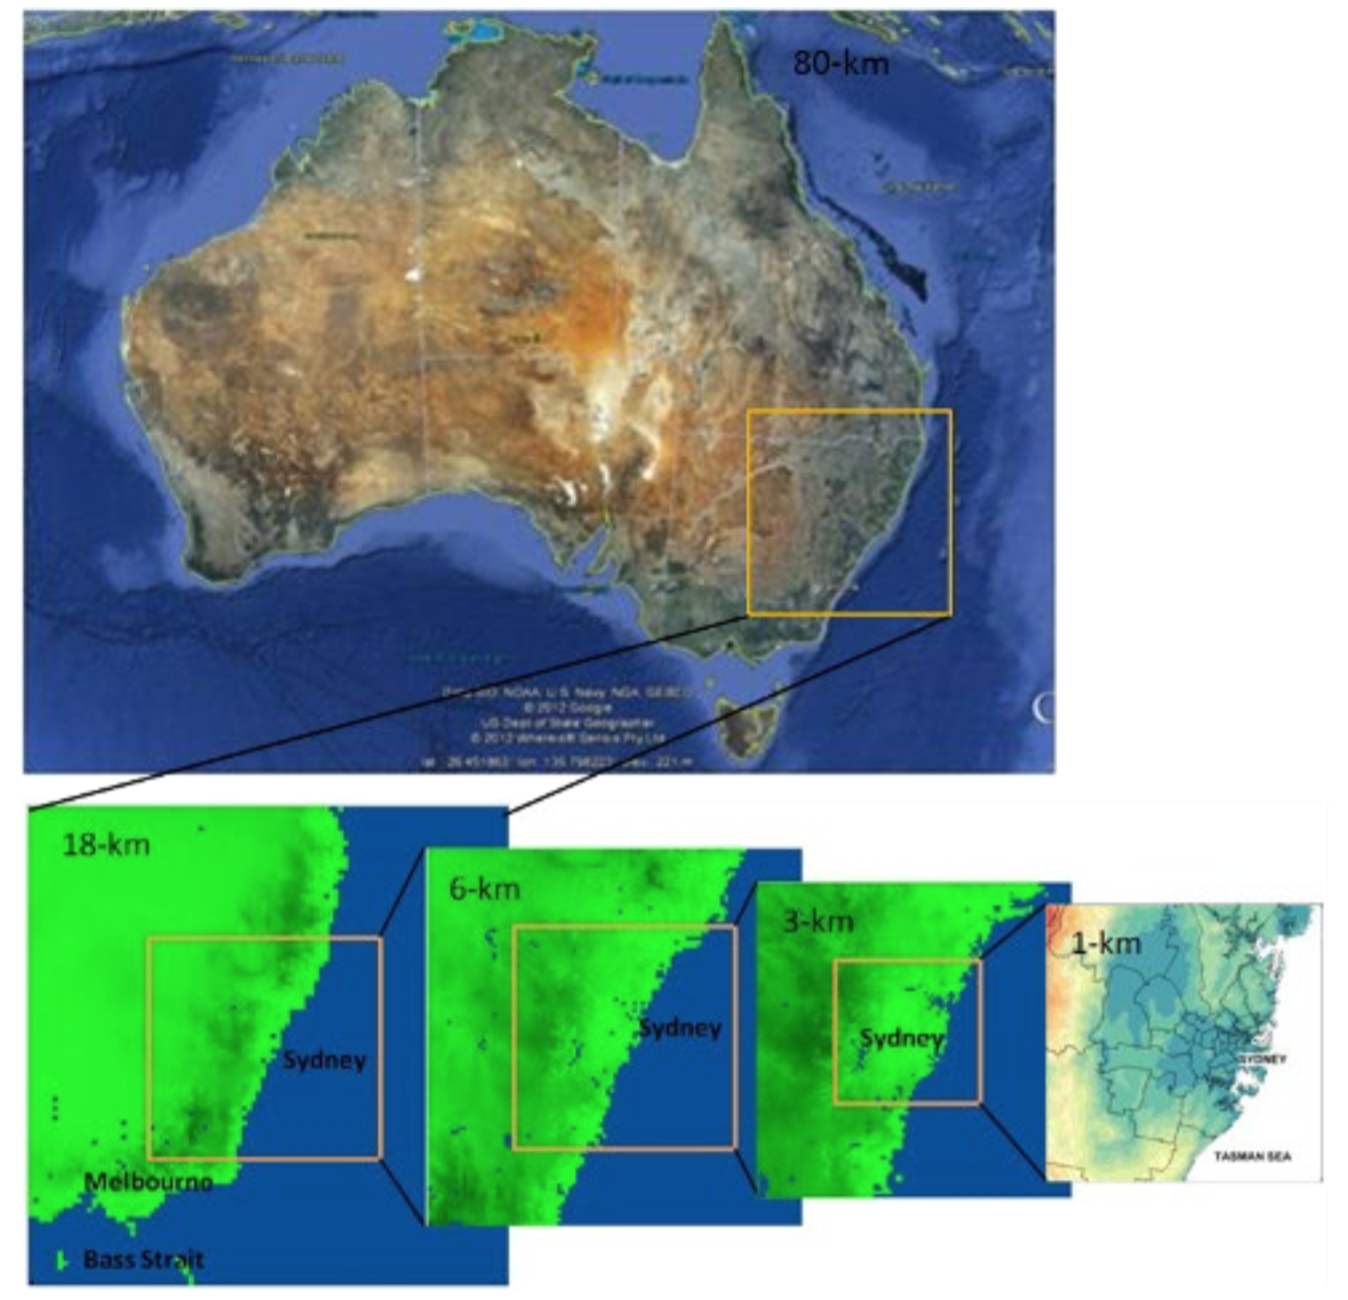
\includegraphics[width=0.8\textwidth,natwidth=1308,natheight=952]{Fig/ctmexample.png}
	    	\caption{A series of the zooming \gls{ctm} grids used in the Sydney Particle Study. An example of a \gls{ctm} produced chemical concentration map can be see at the bottom right \citep{cope:2014tw}.}
	    	\label{fig:sydpartgrid}
		\end{figure}

		\gls{ctm} is written in FORTRAN, but allows for chemical reactions to be entered as regular form chemical equations \citep{cope:2009tz}. It requires a meteorological map as input, along with initial and boundary conditions for each chemical being tracked. Maps for the introduction of chemicals from the surface to the atmosphere are also required, such as when \gls{dms} is produced by the \gls{gbr}. \gls{ctm} outputs atmospheric maps of chemical concentrations.

%--------------------------------------------------------------------------------------------------------------------------%

		\subsection{GLOMAP and GLOMAP-mode}
		\label{subsec:glomap}

		\gls{glomap} is the aerosol micro-physics component of the \gls{ukca} model developed at Leeds university. It uses atmospheric information and chemical concentrations to simulate the large amount of interactions aerosols undergo. It models new particle formation, condensation, cloud processing, hygroscopic growth and many other aerosol processes \citep{mann:2010wb}.

		\gls{glomapm} is an alternate version of \gls{glomap} which segregates aerosols via modes (see \cref{sec:aerosols}) rather than the \gls{glomap}'s direct bin approach. \gls{glomapm} also uses the equilibrium Henry's law style aqueous phase reactions recommended by \citet{barnes:2006ug}, while \gls{glomap} uses a more computationally expensive diffusion limited method \citep{mann:2010wb}. Both differences make \gls{glomapm} less accurate, but also less computationally expensive. Some treatments of particles are also adjusted to better make use of the modal structure. An example is that \gls{glomap} applies rain-out to any particles over \SI{103}{\nm}, while \gls{glomapm} applies rain-out to soluble particles in the accumulation and coarse modes \citep{mann:2010wb}. For modelling \gls{dms} and its aerosol products, \gls{glomap} uses the sulphur oxidation steps outlined in \citet{seinfeld2012atmospheric} and precomputed Henry's law coefficients \citep{mann:2010wb}. 

%'There is a whole section in \citep{Mann:2010wb} that describes the nucleation of new sulfate aerosol. Perhaps you should do an analysis of it comparing its treatment to current research? God this could be a whole section in and of itself... There are a bunch of good references in this section which you can take a look at.'
%Is this method adequate based on the stuff we have already talked about in regard to the sulfur cycle?
% this section might need a boost from "Impact of nucleation on global CCN"

		The chemical concentration maps needed to feed into \gls{glomap} can either be offline, computed beforehand, or online \citep{mann:2010wb}. Online maps are updated by what is consumed or produced within \gls{glomap} and then passed to a chemical transport model running above \gls{glomap} \citep{spracklen2003development}. \gls{glomap} produces maps of aerosol concentrations, separated into bins or modes depending on the version used.

		%there is no aitken mode sea salt produced by the model... from luke

